\documentclass[aip]{revtex4-1}

\setlength{\oddsidemargin}{0in}  %left margin position, reference is one inch
\setlength{\textwidth}{6.5in}    %width of text=8.5-1in-1in for margin
\setlength{\topmargin}{-0.5in}    %reference is at 1.5in, -.5in gives a start of about 1in from top
\setlength{\textheight}{9in}     %length of text=11in-1in-1in (top and bot. marg.) 

\usepackage{amsmath,amssymb}
\usepackage{graphicx}% Include figure files
\usepackage{color}% Include colors for document elements
\usepackage{dcolumn}% Align table columns on decimal point
\usepackage{bm}% bold math

\definecolor{background-color}{gray}{0.98}
\graphicspath{{data/}{images/}}

  \makeatletter
  \renewcommand\@biblabel[1]{#1.}
  \makeatother

\bibliographystyle{apsrev}

\begin{document}

\title{Atomic pseudo-potentials for reproducing the valence electron behaviour of sp$^2$ carbon atoms: Supplementary Material}
\author{Alexander Punter}
\author{Paola Nava}
\author{Yannick Carissan}
\affiliation{Aix Marseille Univ, CNRS, Centrale Marseille, iSm2, Marseille, France}

\maketitle

\subsection{Details on the extraction process}
\subsubsection{CH\(_{3}\), with \(s\) potentials}

We aim first to reproduce the values for the CH\(^{\bullet}_{3}\) radical as given in Table \ref{table:ch3_s_potentials}. 
This reference CH\(^{\bullet}_{3}\) is created and has its geometry optimised under Hartree-Fock (HF/def-SV(P)). The reference geometry gives a C - H distance of 2.0466 a.u., and so we pick \(d = 2.0\) a.u. as a starting guess for the planar distance from the pseudo-carbon, \(d\), of our pseudo-potentials. The pseudo-system is then set up, erasing the hydrogen atoms, setting the carbon charge \(Z_{nucleus} = 1\) and applying \(s\) pseudo-potentials, as well as selecting the correct orbital for the remaining electron. Table \ref{table:ch3_s_potentials} displays some of our results. Promisingly, we are able to produce many sets of potentials that give the correct energy.

\subsubsection{Ethene, with \(s\) and \(p\) potentials}

Next, we take some of these potentials to create a pseudo-ethene system, with the results shown in Table \ref{table:ethene_s_pseudo}. All potentials tested with \(d = 2.0\) a.u. gave results several orders of magnitude away from the reference value. From Figure \ref{fig:long_r_ethene} we may see the reason. One of the potential sets from each carbon is closer to the neighbouring carbon than the neighbour's own potential sets, thus both pseudo-carbons are affected by potentials which do not belong to them. At the shorter range \(d = 0.5\) a.u., the HOMO energy is of the right magnitude, though with errors of \(~ 30\%\). Attempts to eliminate this error lead us to the additional use of the \(p_{z}\) potential \textit{alongside} the \(s\) potentials.

The next step adds a \(p\) potential centred on the pseudo-carbon, with Table \ref{table:p_potentials} displaying the results. As before, \(d = 0.5\) a.u.. The \(p_{z}\) potential is selected using the procedure described in Section II B, with the exponent chosen to give the maximum possible overlap with the \(p_{z}\) orbital, and the matching \(Z_{eff}\) coefficient calculated from the exponent and overlap. The \(s\) potentials are then optimised once more to give the correct HOMO energy for CH\(^{\bullet}_{3}\). We again take these potentials to create a pseudo-ethene molecule, with the results shown in Table \ref{table:p_potentials}. We can see that these potentials seem to transfer more effectively from the CH\(^{\bullet}_{3}\) system to the ethene, suggesting therefore that whilst the \(s\) potentials can affect both the \(p_{z}\) and \(\pi\) orbitals, they 
cannot alone describe the relationship between them.

Having successfully created a pseudo-ethene with the correct HOMO, we attempt to have the pseudo-system replicate other properties of the real system:
the singlet-triplet excitation energy ($\Delta_{ST}$) in the SCF framework (energy difference between the triplet and the singlet mono-reference
calculations), the ionisation energy (IE) and the energy of the HOMO orbital ($\varepsilon_{HOMO}$). Reference values for the singlet-triplet \(\pi-\pi^{*}\) excitation and first ionisation energies of ethene are given in Table III. Testing the relevant energies for the optimised pseudo-systems above, we found that the early results were not promising. However, after we abandon the notion of sticking strictly to a \(p_{z}\) potential exponent that gives the maximum overlap with the real orbital, we discover there is a "sweet spot" of potential coefficients and exponents around which the correct values begin to emerge. Tables II and III show our optimal result, chosen to give HOMO, ($\Delta_{ST}$) and ionisation energies closest to the reference values. 

\subsubsection{Optimisation}

In earlier calculations with only \(s\) potentials, optimisation was performed by choosing a range of exponent values and attempting to optimise the coefficient at each to produce the HOMO reference energy. Once the \(p_{z}\) potential was added, the \(s\) potentials were optimised afterward. 

Once we started to look at excitation and ionisation energies however, optimisation became more complicated. Optimisations were at first performed of the $s$ and $p$ potentials to reach the HOMO energy of ethene as before. With the different potential variables available, we produced a range of optimised potential sets. The best set of these potentials was then chosen and the values altered by hand in order to match as closely as possible three separate reference values: the singlet HOMO energy, the singlet-triplet \(\pi-\pi^{*}\) excitation energy, and the cation-singlet energy. All optimisations used the Brent method in SciPy's optimisation library, with a tolerance of \(1.48*10^{-08}\), and used standard Hartree-Fock calculations.

\subsection{Comparison with our previous study}
\begin{figure}
\begin{center}
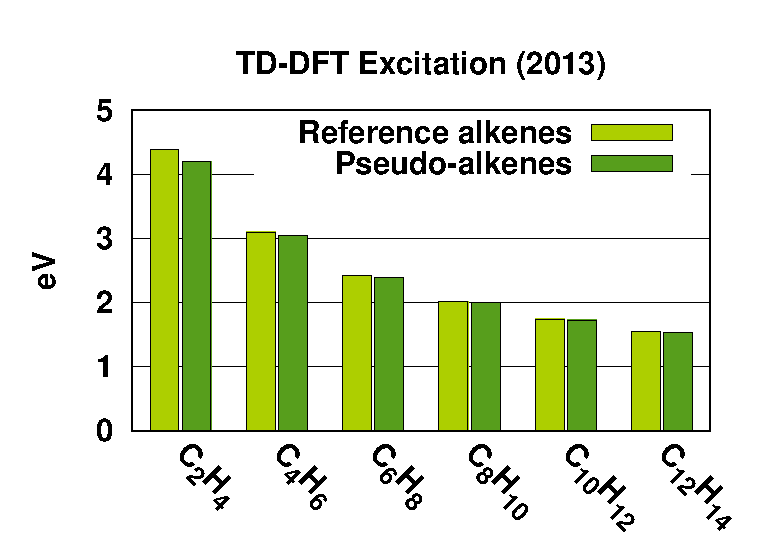
\includegraphics[width=8cm]{short_pbe0_tddft_2013}
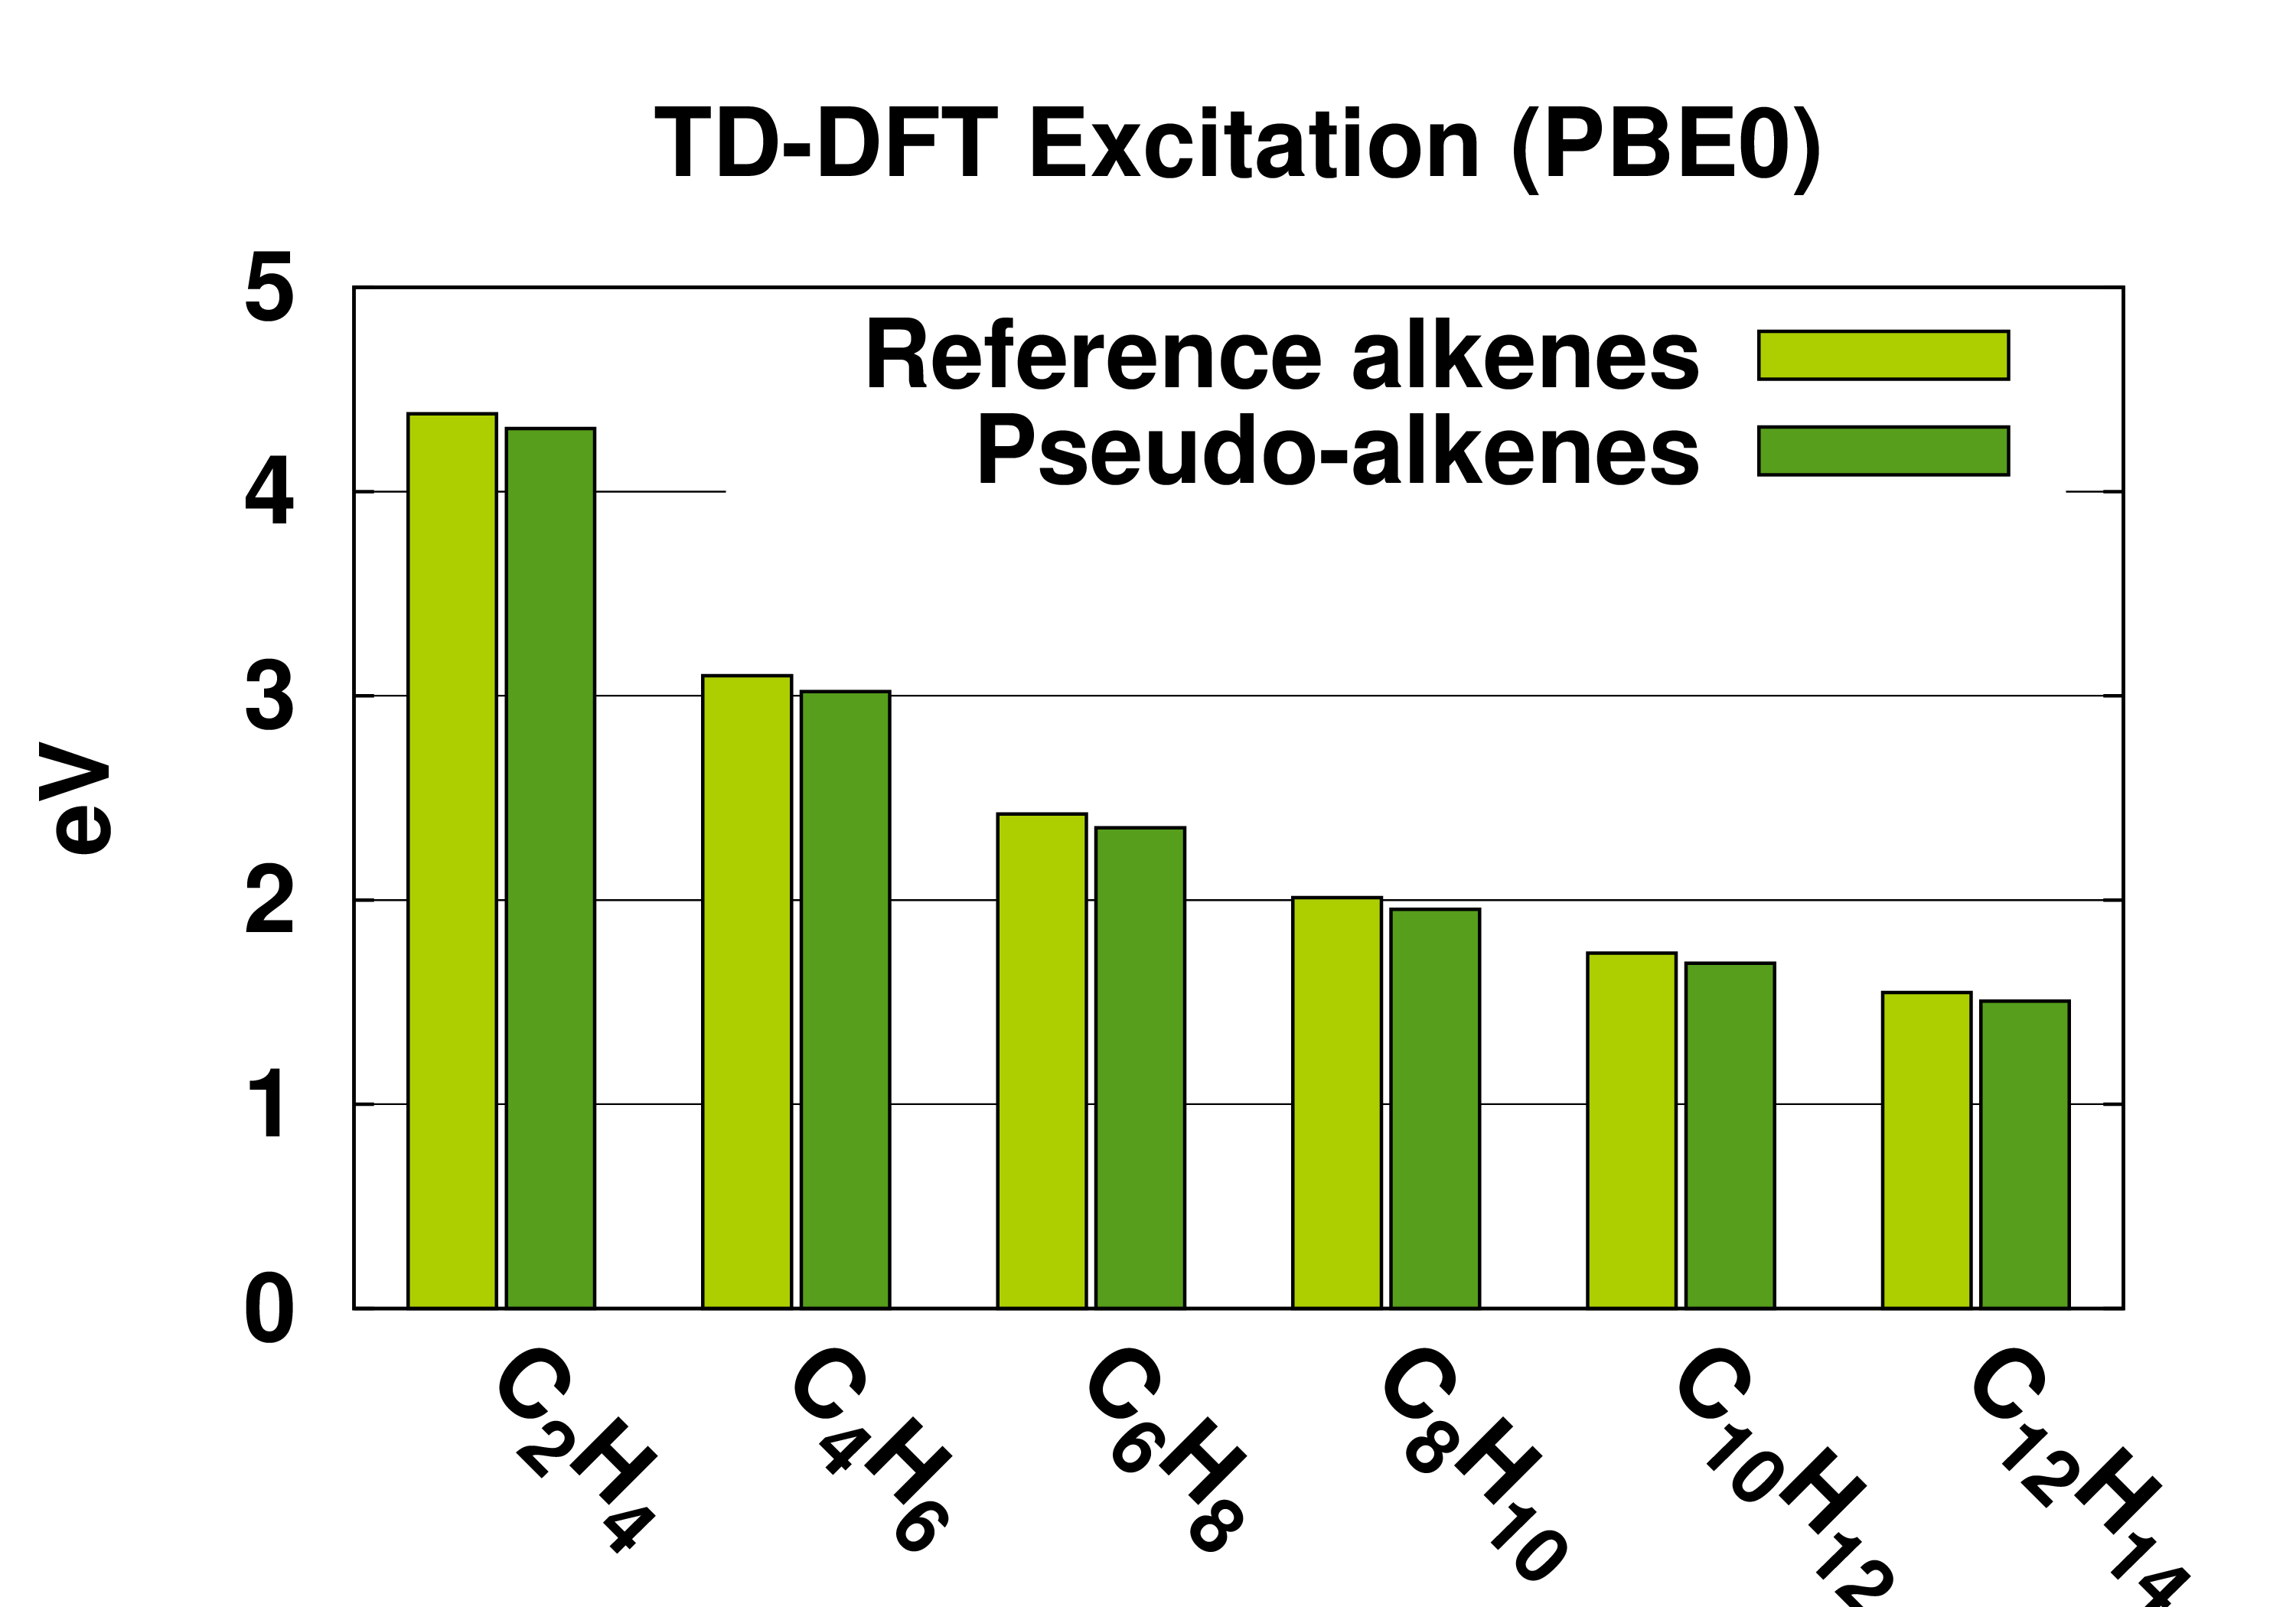
\includegraphics[width=8cm]{short_pbe0_tddft}
\end{center}
\caption{Comparison of pseudo-alkenes with previous (Drujon and Carissan, JCC 2013 (34) 49-59) and current potentials using TD-DFT excitation energies.}
\label{fig:alkenes_tddft}
\end{figure}

%%%%%%%%%%%%%%%%%%%%%%%%%%%%%%%%%%%%%%%%%%%%%%%%%%%%%%%%%%%%%%%%%%%%%%%%%%%%%%%%%
% FIGURE CAPTIONS

%%%%% FIGURE ---- cc.eps
\begin{figure}
\begin{center}
%\includegraphics[width=0.2\columnwidth,keepaspectratio=true]{cc.eps}
\fbox{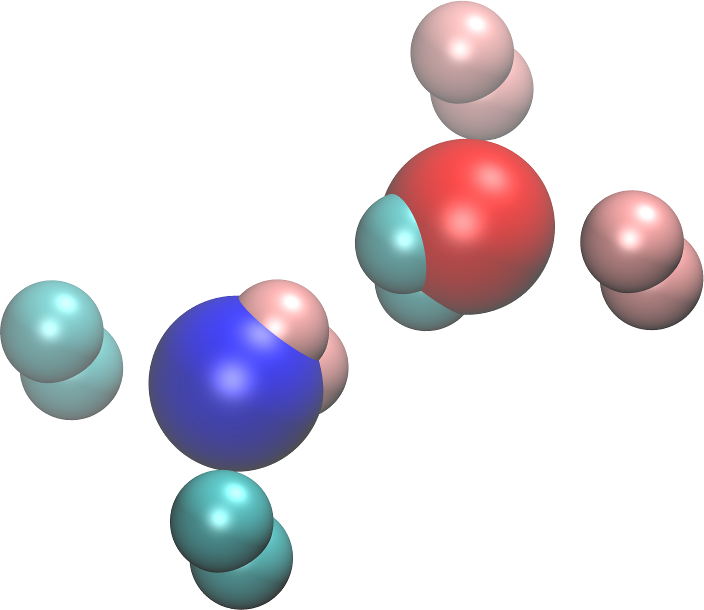
\includegraphics[width=0.45\textwidth]{hires_long_r_crop.png}}%
\fbox{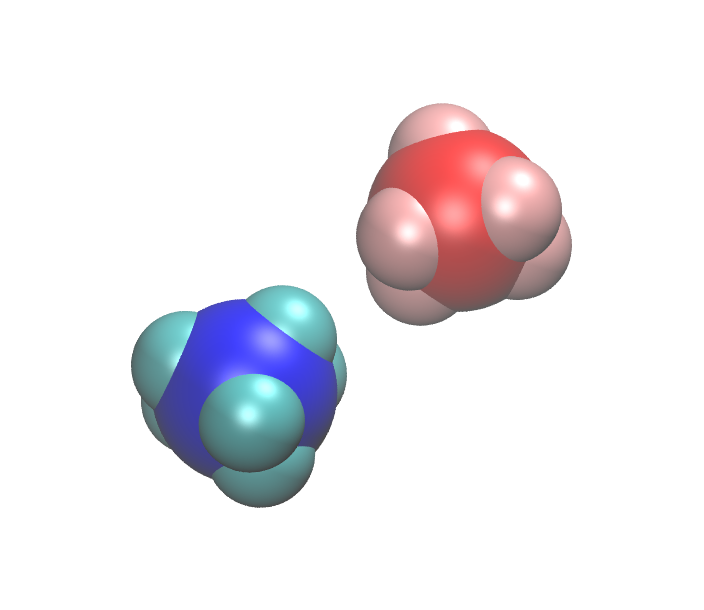
\includegraphics[width=0.45\textwidth]{hires_short_r_crop.png}}
\end{center}
\caption{Diagrams of pseudo-ethene with \(d =\) 2.0 a.u. (left), and \(d = 0.5\) a.u. (right). The first pseudo-carbon is displayed in blue, with its \(s\) pseudo-potentials in cyan, and the second pseudo-carbon is in red, with its potentials in pink.}
\label{fig:long_r_ethene}
\end{figure}
%%%%%%%%%%%%%%%%%%%%%%%%%%%%
\clearpage

\begin{table}[ht]
\begin{tabular}{c c c}
\hline\hline
 & Coefficient & Exponent \\ 
\hline
HF & -2.594 & 1.0 \\
 & -4.788 & 5.0 \\
 & -7.524 & 10.0 \\
\hline
PBE0 & -2.605 & 1.0 \\
 & -4.873 & 5.0 \\
 & -7.678 & 10.0 \\
\hline\hline
\end{tabular}
\caption{Coefficients and exponents for \(s\)-only pseudo-potentials for CH\(^{\bullet}_{3}\), optimised to give 
the all-electron HOMO reference energy of  -10.537~eV (HF) and -6.726~eV (PBE0). 
\(d = 0.5\) a.u., as defined in Figure 1.}
\label{table:ch3_s_potentials}
\end{table}

\newpage

\begin{table}[ht]
\begin{tabular}{c c c c}
\hline\hline
& $d$ & \(s\) coefficient & \( \pi \)  \\
\hline
HF$^a$   &     &        & -10.363 \\
PBE0$^a$ &     &        & -6.632 \\
HF       & 2.0 & -7.521 & -9597.0 \\
HF       & 0.5 & -7.521  & -7.905 \\
PBE0     & 0.5 &-7.678  & -8.447 \\
\hline\hline
\multicolumn{4}{l}{$^a$ All-electron reference values.}\\
\end{tabular}
\caption{HOMO energies ($\pi$, eV) for ethene and pseudo-ethene. The pseudo-potentials used in the pseudo-ethene are taken from optimised values for 
pseudo-CH\(^{\bullet}_{3}\) with only \(s\) potentials and an exponent of 10.0. $d$ (a.u.) as defined 
in Figure 1.}
\label{table:ethene_s_pseudo}
\end{table}

\newpage

\begin{table}[ht]
\begin{tabular}{c c c c}
\hline\hline
& \(p\) coefficient & \(p\) exponent \\
\hline
\(p_{z}\) potential & -3.267 & 0.295 \\
\hline
Calculation Type & \(s\) coefficient & \(s\) exponent & \(\pi\) \\
\hline
HF & 2.772 & 1.0 & -13.654 \\
 & 6.173 & 5.0 & -14.011 \\
 & 10.381 & 10.0 & -14.061 \\
\hline
PBE0 & 3.483 & 1.0 & -10.325 \\
 & 9.801 & 5.0 & -10.409 \\
 & 18.351 & 10.0 & -12.543 \\
\hline\hline
\end{tabular}
\caption{\(\pi\) orbital energy values (eV) for pseudo-ethene, using \(s\) and \(p\) pseudo-potentials.
The pseudo-potentials are taken from a pseudo-CH\(^{\bullet}_{3}\) system optimised to give the correct all-electron HOMO energy.}
\label{table:p_potentials}
\end{table}

\subsection{Timings}
The reduction of computational time necessary for calculations was not our primary aim, however the model that we develop in this work does allow significant gains.
To illustrate this, we provide in Table \ref{tab:time} a small study done on the C$_{50}$H$_{52}$
alkene chain.
Calculations were performed with two different basis sets: def2-SV(P) and QZVPPD.
When using the pseudo-potential, the basis set was truncated by removing all
basis functions not necessary to reproduce the
$\pi$ system.
In other words, only $p$ functions or those of higher angular momentum were kept.
As can be seen from Table \ref{tab:time}, the gain increases
with the size of the basis set as expected.
The gain ranges from 3 (def2-SV(P)) to 8 (QZVPPD).

\begin{table}[ht]
\begin{tabular}{lrr}
\hline\hline
Model            & def2-SV(P) & QZVPP \\
\hline
All electrons    &        67 & 68928 \\
Pseudo-potential &        28 &  8566 \\
Gain             &       2.4 &   8.0 \\
\hline\hline
\end{tabular}
\caption{\label{tab:time}Time (in seconds) per SCF iteration.} 
\end{table}

\bibliography{biblio_pseudo_alex} 

\end{document}
